%%%%%%%%%%%%%%%%%%%%%%%%%%%%%%%%%%%
%This is the LaTeX ARTICLE template for RSC journals
%Copyright The Royal Society of Chemistry 2016
%%%%%%%%%%%%%%%%%%%%%%%%%%%%%%%%%%%

\documentclass[twoside,twocolumn,9pt]{article}

\usepackage{tgheros}
\renewcommand{\familydefault}{\sfdefault}

\usepackage{extsizes}
\usepackage[super,sort&compress,comma]{natbib}
\usepackage[version=3]{mhchem}
\usepackage[left=1.5cm, right=1.5cm, top=1.785cm, bottom=2.0cm]{geometry}
\usepackage{balance}
\usepackage{mathptmx}
\usepackage{mathtools}
\usepackage{amsfonts}
\usepackage{sectsty}
\usepackage{graphicx}
\usepackage{lastpage}
\usepackage[format=plain,justification=justified,singlelinecheck=false,font={stretch=1.125,small,sf},labelfont=bf,labelsep=space]{caption}
\usepackage{float}
\usepackage{fancyhdr}
\usepackage{fnpos}
\usepackage[english]{babel}
\addto{\cuptionsenglish}{%
	\renewcommand{\refname}{Notes and references}
}
\usepackage{array}
\usepackage{droidsans}
\usepackage{charter}
\usepackage[T1]{fontenc}
\usepackage[usenames,dvipsnames]{xcolor}
\usepackage{setspace}
\usepackage[compact]{titlesec}
%%%Please don't disable any packages in the preamble, as this may cause the template to display incorrectly.%%%


\usepackage{xcolor}
\definecolor{ugent_blue}{RGB}{30, 100, 200}
\definecolor{ugent_yellow}{cmyk}{.0, .10, 1, 0}

\usepackage{titlesec}
\titleformat{\section}
{\color{black}\normalfont\Large\bfseries}
{\color{black}\thesection}{1em}{}

\usepackage[colorlinks=true,linkcolor=black,citecolor=ugent_blue]{hyperref}

%\AtEveryCite{\color{ugent_blue}}




\usepackage{epstopdf}%This line makes .eps figures into .pdf - please comment out if not required.
\usepackage{physics}
\usepackage{cleveref}
\usepackage{booktabs}
\usepackage{pdfpages}

\definecolor{cream}{RGB}{222,217,201}

\begin{document}

\pagestyle{fancy}
\thispagestyle{plain}
\fancypagestyle{plain}{
	%%%HEADER%%%
	\renewcommand{\headrulewidth}{0pt}
}
%%%END OF HEADER%%%

%%%PAGE SETUP - Please do not change any commands within this section%%%
\makeFNbottom
\makeatletter
\renewcommand\LARGE{\@setfontsize\LARGE{15pt}{17}}
\renewcommand\Large{\@setfontsize\Large{12pt}{14}}
\renewcommand\large{\@setfontsize\large{10pt}{12}}
\renewcommand\footnotesize{\@setfontsize\footnotesize{7pt}{10}}
\makeatother

\renewcommand{\thefootnote}{\fnsymbol{footnote}}
\renewcommand\footnoterule{\vspace*{1pt}% 
	\color{cream}\hrule width 3.5in height 0.4pt \color{black}\vspace*{5pt}}
\setcounter{secnumdepth}{5}

\makeatletter
\renewcommand\@biblabel[1]{#1}
\renewcommand\@makefntext[1]% 
{\noindent\makebox[0pt][r]{\@thefnmark\,}#1}
\makeatother
\renewcommand{\figurename}{\small{Fig.}~}
\sectionfont{\sffamily\Large}
\subsectionfont{\normalsize}
\subsubsectionfont{\bf}
\setstretch{1.125} %In particular, please do not alter this line.
\setlength{\skip\footins}{0.8cm}
\setlength{\footnotesep}{0.25cm}
\setlength{\jot}{10pt}
\titlespacing*{\section}{0pt}{4pt}{4pt}
\titlespacing*{\subsection}{0pt}{15pt}{1pt}
%%%END OF PAGE SETUP%%%

%%%FOOTER%%%
\fancyfoot{}
\fancyfoot[LO,RE]{\vspace{-7.1pt}\includegraphics[height=9pt]{head_foot/LF}}
\fancyfoot[RO]{\footnotesize{\sffamily{1--\pageref{LastPage} {\color{ugent_yellow} ~\textbar } \hspace{2pt}\thepage}}}
\fancyfoot[LE]{\footnotesize{\sffamily{\thepage~{\color{ugent_yellow} ~\textbar }\hspace{4.65cm} 1--\pageref{LastPage}}}}
\fancyhead{}
\renewcommand{\headrulewidth}{0pt}
\renewcommand{\footrulewidth}{0pt}
\setlength{\arrayrulewidth}{1pt}
\setlength{\columnsep}{6.5mm}
\setlength\bibsep{1pt}
%%%END OF FOOTER%%%

%%%FIGURE SETUP - please do not change any commands within this section%%%
\makeatletter
\newlength{\figrulesep}
\setlength{\figrulesep}{0.5\textfloatsep}

\newcommand{\topfigrule}{\vspace*{-1pt}% 
	\noindent{\color{cream}\rule[-\figrulesep]{\columnwidth}{1.5pt}} }

\newcommand{\botfigrule}{\vspace*{-2pt}% 
	\noindent{\color{cream}\rule[\figrulesep]{\columnwidth}{1.5pt}} }

\newcommand{\dblfigrule}{\vspace*{-1pt}% 
	\noindent{\color{cream}\rule[-\figrulesep]{\textwidth}{1.5pt}} }

\makeatother
%%%END OF FIGURE SETUP%%%

%%%TITLE, AUTHORS AND ABSTRACT%%%
\twocolumn[
	\begin{@twocolumnfalse}
		{
			\includegraphics[width=18.5cm]{head_foot/header_bar}}\par
		\vspace{1em}
		\sffamily
		\begin{tabular}{m{4.5cm} p{13.5cm} }

			               & \noindent\LARGE{\textbf{Explainable graph neural networks $^\dag$}}                                             \\%Article title goes here instead of the text "This is the title"
			\vspace{0.3cm} & \vspace{0.3cm}                                                                                                  \\

			               & \noindent\large{Full Name,$^{\ast}$\textit{$^{a}$} Full Name,\textit{$^{b\ddag}$} and Full Name\textit{$^{a}$}} \\%Author names go here instead of "Full name", etc.

			               &                                                                                                                 \\

			               & \noindent\normalsize{abstract}                                                                                  \\%The abstrast goes here instead of the text "The abstract should be..."
		\end{tabular}

	\end{@twocolumnfalse} \vspace{1.6cm}

]
%%%END OF TITLE, AUTHORS AND ABSTRACT%%%

%%%FONT SETUP - please do not change any commands within this section
\renewcommand*\rmdefault{bch}\normalfont\upshape
\rmfamily
\section*{}
\vspace{-1cm}


% %%%FOOTNOTES%%%

\footnotetext{\textit{$^{b}$~Corresponding author:} \texttt{firstname.lastname@ugent.be}}

% %Please use \dag to cite the ESI in the main text of the article.
% %If you article does not have ESI please remove the the \dag symbol from the title and the footnotetext below.
% \footnotetext{\dag~Electronic Supplementary Information (ESI) available: [details of any supplementary information available should be included here]. See DOI: 00.0000/00000000.}
% %additional addresses can be cited as above using the lower-case letters, c, d, e... If all authors are from the same address, no letter is required

% \footnotetext{\ddag~Additional footnotes to the title and authors can be included \textit{e.g.}\ `Present address:' or `These authors contributed equally to this work' as above using the symbols: \ddag, \textsection, and \P. Please place the appropriate symbol next to the author's name and include a \texttt{\textbackslash footnotetext} entry in the the correct place in the list.}


%%%END OF FOOTNOTES%%%

%%%MAIN TEXT%%%%

\section{Introduction}
% Central ideas: Why did I do the work? What were the central motivations and hypotheses?

% The first paragraph or two should be written out completely. Pay particular attention to the opening sentence. Ideally, it should state concisely the objective of the work, and indicate why this objective is important.
% In general, the Introduction should have these elements: 

% \begin{itemize}
%     \item The objectives of the work. 
%     \item The justification for these objectives: Why is the work important? Cite the most important works \cite{whitesides2004a}.
%     \item Background: Who else has done what? How? What have we done previously?
%     \item Guidance to the reader: What should the reader watch for in the paper? What are the interesting high points? What strategy did we use?
%     \item Summary/conclusion: What should the reader expect as conclusion? In advanced versions of the outline, you should also include all the sections that will go in the Experimental section (at the level of paragraph subheadings) and indicate what information will go in the Microfilm section.
% \end{itemize}

\begin{itemize}

    \item Although machine learning (ML) models are able to achieve remarkable accurate results in,
        for example, molecule property prediction\cite{}, synthetic path way design\cite{}, 
        inverse molecular design\cite{} ..., their predictions are opaque.\cite{} This lack 
        of explainability creates trust issues when those ML models are used in performance critical 
        and/or highly regulated environment such as drug discovery.\cite{} Also, potential novel 
        scientific insights learned by the model remain hidden inside the black box.\cite{carvalho2019machine}

	\item Explainable artificial intelligence (XAI) uses different approaches to uncover the black 
        box nature of ML models, resulting in more trusted models.\cite{carvalho2019machine} Using the taxonomy of 
        Yuan et. al., there are five classes of XAI methods: gradient based, perturbation, surrogate, 
        decomposition and generation.\cite{yuan2022explainability} However, all fail to give an explanation which is 
        intuitive for chemists.

    \item Recently, Wu et. al used substructure mask exploration to explain molecular property models 
        in a chemically intuitive manner.\cite{wu2023chemistry} Their approach uses the difference between the prediction
	      of a molecule and the prediction when a functional group of that molecule is removed.
	      An additional benefit of this method is that a linear model can be fitted to optimize
	      molecular properties without the need of training an expensive machine learning model.

	\item However, just using the difference could lead to wrong interpretations due to interaction
	      effects. A commonly used method to fairly distribute the prediction over the
          features is the Shapley value\cite{shapley1953value} taken from cooperative game theory.\cite{molnar2020interpretable} This value cannot
	      be applied in the context of GNN as the Shapley value does not take the graphical structure
	      into account. Therefore the structure aware HM-value is used instead.\cite{hamiache_value_1999, hamiache_associated_2020}
\end{itemize}


\section{Theory}

\subsection{The Shapley value}

The Shapley value is originally designed in cooperative game theory.\cite{shapley1953value} Cooperative
game theory is interested into how much each player has participated to obtain a certain
result (i.e. pay-off).\cite{branzei2008models} This can be translated to ML by treating the features 
as the players and the model prediction as the pay-off.\cite{merrick2020explanation}

A game with transfer utility (i.e. TU-game) is defined as a pair $\left(N, v\right)$ of a set
of players $N$ and a characteristic function $v$ which satisfies\cite{branzei2008models}

\begin{equation}
	v: 2^N \coloneqq \{S | S \subseteq N\} \rightarrow \mathbb{R}, \; v\left(\emptyset\right) = 0.
\end{equation}

The pay-off of a coalition (i.e. set of players) is determined by the characteristic
function. The marginal contribution of player $i$ is defined as\cite{zhang2022gstarx}

\begin{equation}
	m(i) = v\left(S \cup \{i\}\right) - v\left(S\right), \; \text{with } S \subseteq N \textbackslash \{i\}.
\end{equation}

The Shapley value $\phi_i$ of player $i$ is computed as a double average over all marginal contributions\cite{zhang2022gstarx}

\begin{equation}
	\label{eq:Shapley}
        \phi_i  = \frac{1}{|N|} \sum_{k=0}^{|N|-1} \frac{\left(|N| - 1 - k\right)k!}{\left(|N| - 1\right)!} \sum_{S \subseteq N \textbackslash \{i\}, |S| = k} m(i). 
\end{equation}

There are $|N|$ coalitions with different sizes and ${|N| - 1 \choose k}$ coalitions of size $k$.
When the summations are rearranged and substituting $k$ with $|S|$, both weights can be combined 
resulting in 

\begin{equation}
	\phi_i = \sum_{S \subseteq N \textbackslash \{i\}} \frac{\left(|N| - 1 - |S| \right)!|S|!}{|N|!} m(i).
\end{equation}

A limitation of the Shapley value is that every coalition is considered.\cite{zhang2022gstarx} 
However, consider a graph neural network where the interest of explanation lies in the detection 
of the most important nodes or super nodes. In this case some coalitions are impossible. To solve 
this restriction, values on games with incomplete communication\cite{myerson1977graphs} are explored. 
Games with incomplete communication use a graph to represent which players can communicate with each other.
One value was developed by Hamiache and Navarro.\cite{hamiache_value_1999, hamiache_associated_2020}.

\subsection{The Hamiache Navarro value}

Let a game $(N, v)$ with a communication structure be a triple $(N, v, g)$, where $g$ is
set of adjacent nodes\cite{hamiache_value_1999},

\begin{equation}
	g \subseteq g_N \coloneq \{ \{i, j \} | i, j \in N \}
\end{equation}

The graph $\left< N, g \right>$ specifies the communication structure, where only adjacent
players (i.e. $i$ and $j$ are adjacent if and only if $\{ i, j \} \in g$) are allowed to
communicate with each other. Define a path as a sequence $i = i_1, i_2, \dots, i_k = j$
of nodes from player $i$ to player $j$ such that

\begin{equation}
	\{i_q, i_{q+1} \} \in g, \; 1 \le q \le k - 1.
\end{equation}

If such a path exists between two players, then they are connected which is denoted by
$i \underset{\left< N, g \right>}{\rightarrow} j$. The partion $N/g$ of the set of
nodes $N$ over the graph $\left< N, g \right>$ is than the set of all connected nodes

\begin{equation}
N/g = \{\{ i | i \in N \land i \underset{\left<N, g \right>}{\rightarrow} j\} \cup \{j\} | j \in N \}.
\end{equation}

A coalitions $S \subseteq N$ can only directly interact with its connected neighbours. Let 
$S^*$ be the set of players in the coalition $S$ together with their connected neighbours, 

\begin{equation}
    S^* \coloneqq \{ i \in N | \exists j \in S \text{ such that } \{i, j\} \in g \} \cup S.
\end{equation}

The associated game $(N, v^*, g)$ of $(N, v, g)$ given a real number $\tau$ is defined by 

\begin{equation}
    v^*(S) = 
    \begin{cases}
        v(S) + \tau \sum_{j \in \mathcal{N}(S)} \left[ v(S \cup \{j\}) - v(S) - v(\{j\}) \right]  & \text{if } |S/g| = 1 \\
        \sum_{R \in S/g} v^*(R) &  \text{otherwise}
    \end{cases}
    .
\end{equation}

A matrix representation of the associated game is obtained by defining the matrices $M_c$, 

\begin{equation}
    M_c[S, T] = 
    \begin{cases} 
        1 - |N \textbackslash S| \tau & \text{if } |S| = |T| \\
        \tau & \text{if } |S| + 1 = |T| \land S \subseteq T \\
        -\tau & \text{if } |T| = 1  \land T \not \subseteq S \\
        0 & \text{otherwise}
    \end{cases}
\end{equation}

and $P_g$,

\begin{equation}
    P_g[S, T] = 
    \begin{cases} 
        1 & \text{if } T \in S/g \\
        0 & \text{otherwise} \\
    \end{cases}
\end{equation}

\subsection{Substructure mask exploration}







\section{Methodology}


\newpage
\section{Results and discussion}


\subsection{Evaluation metrics}

\subsubsection{Spearman rank correlation with chemicaly intuitively ranked substructures}

\begin{center}
\begin{table}[H]
    \caption{Average Spearman rank correlation between the attributions and chemical intuitive ranks. Molecules where 
        subdivided into two groups based on whether the absolute difference between the corresponding model prediction 
        and the experimental value is below $0.6$logS.
    }
\begin{tabular}{lrrr}
\toprule
 & SME  & Shapley  & HN  \\
absolute error &  &  &  \\
\midrule
< 0.6 & 0.765754 & 0.750960 & 0.740930 \\
>= 0.6 & 0.522455 & 0.543093 & 0.534330 \\
 \bottomrule
\end{tabular}
\end{table}
\end{center}


To analyse which attribution method provides the most accurate
explanation, the Spearman rank correlation is computed between the
substructures attributions and a chemically intuitive ranking of those
substructures. Also the influence of the absolute error between model
prediction and experimental value will be examined by subdividing the
molecules into two \((<0.6\) or \(>=0.6)\). Since the distributions of
the Spearman rank correlations are highly skewed to the left,
non-parametric test are used for the analysis. To test whether there is
a significant difference of rank correlation between the attribution
methods two Friedman test will be used (one for each absolute error
category). For testing the presence of a significant difference between
the AE groups a three Wilcoxon--Mann--Whitney test will be applied.
Control for the multiple test will be done using Bonferonni, resulting
in a significance level of \(0.05/5 = 0.01\).


\begin{figure}[H]
    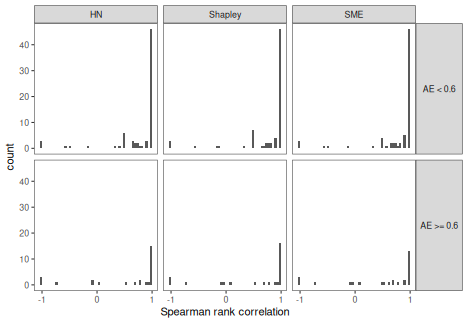
\includegraphics[scale=0.5]{./distributions-1.png}
\end{figure}


\textbf{Friedman test of attribution methods}
\label{friedman-test-of-attribution-methods}


The presence of a statistical difference in Spearman rank correlation
between attributions and chemically intuitive ranks for different
attribution methods is tested using a Friedman test. The null-hypothesis
assumes that there is no difference between the different attribution
methods, which would result in similar rank sums of the different
attribution methods. For both groups of absolute error, smaller than
\(0.6\) (p-value 0.217) and larger than or equal to \(0.6\) (p-value
0.152), are not significant based on the bonferonni corrected nominal
level of \(0.01\). Therefore, it is concluded that there is not enough
evidence in the data to reject the null hypothesis and it is assumened
the the method of computing the attribution values has not a significant
impact in the accurateness of the resulting explanation.




\begin{center}
    \begin{table}[H]
        \caption{
Friedman test result for molecules with absolute prediction
error smaller than \(0.6\)}
\begin{tabular}{lrrrrl}
\toprule
 n & statistic & df & p & method \\
\midrule
 72 & 3.058823 & 2 & 0.2166631 & Friedman test \\
\bottomrule
\end{tabular}
\end{table}
\end{center}




\begin{center}
    \begin{table}[H]
        \caption{
Friedman test result for molecules with absolute prediction
error larger than or equal to \(0.6\)}
\begin{tabular}{lrrrrl}
\toprule
n & statistic & df & p & method \\
\midrule
28 & 3.769231 & 2 & 0.1518875 & Friedman test \\
\bottomrule
\end{tabular}
\end{table}
\end{center}


\textbf{Wilcoxon-Mann-Whitney test between absolute error groups}


In all attribution methods there is no significance difference between the two different
absolute error groups (p-values are 0.035, 0.281, 0.145 for SME, Shapley
and HN respectively ). Therefore, it is concluded that there is not enough evidence in
the data to reject the null hypothesis of equal distributions.

\begin{center}
    \begin{table}[H]
        \begin{tabular}{lcccl}
            \toprule
            &SME & Shapley & HN \\
            \midrule 
        W & 1254.5 & 1132 &  1177.5 \\
        p &  0.035 & 0.281 & 0.145 \\
        \bottomrule
    \end{tabular}
\end{table}
\end{center}


\subsubsection{Fidelity}

Fidelity measures how faithfull the explanations are to the model. 
Most positive fidelities are negative, meaning that removing the most important 
substructure results in an increase in the predicted water solubility.

\begin{center}
    \begin{table}[H]
        \caption{Average positive and negative fidelity in logS for test data set (100 molecules)}
\begin{tabular}{lrrr}
\toprule
 & SME & Shapley  & HN \\
\midrule
Fidelity+ & 2.35 & 2.34 & 2.32 \\
Fidelity- & 0.39 & 0.43 & 0.43 \\
 \bottomrule
\end{tabular}
\end{table}
\end{center}

\begin{figure}[H]
    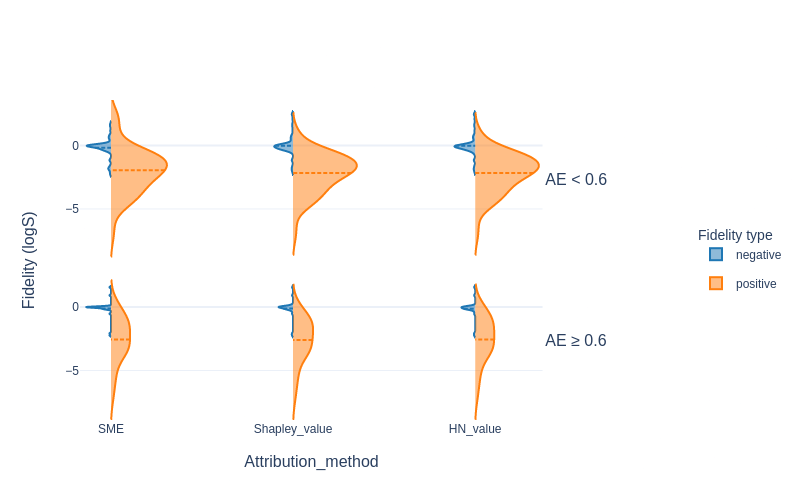
\includegraphics[scale=0.35]{../data/images/esol_fidelity_distributions.png}
\end{figure}


\section{Conclusions}

%%%END OF MAIN TEXT%%%

%The \balance command can be used to balance the columns on the final page if desired. It should be placed anywhere within the first column of the last page.

\balance

%If notes are included in your references you can change the title from 'References' to 'Notes and references' using the following command:
%\renewcommand\refname{Notes and references}

%%%REFERENCES%%%
\bibliography{outline} %You need to replace "rsc" on this line with the name of your .bib file
\bibliographystyle{aip} %the AIP's .bst file

\newpage
\appendix
\markboth{Appendix}{}
\renewcommand{\thesection}{A.\arabic{section}}



\end{document}
